\documentclass[10pt,a4paper]{article}

\usepackage[utf8]{inputenc}
\usepackage{lmodern}
\usepackage[margin=0.62in]{geometry}
\usepackage{amsmath,amssymb}
\usepackage{booktabs}
\usepackage{graphicx}
\usepackage{xcolor}
\usepackage{hyperref}
\usepackage{tikz}
\usepackage{subcaption}
\usepackage{enumitem}
\usepackage{microtype}
\usepackage{fancyhdr}
\usepackage{titlesec}
\usepackage{tabularx}

\titlespacing*{\section}{0pt}{0.9ex plus 0.2ex minus .1ex}{0.35ex plus .1ex}
\titlespacing*{\subsection}{0pt}{0.6ex plus 0.2ex minus .1ex}{0.25ex plus .1ex}
\titleformat*{\section}{\large\bfseries\color{ugmblue}}
\titleformat*{\subsection}{\normalsize\bfseries}
\setlist{nosep,topsep=0.1em,partopsep=0em,parsep=0.02em,itemsep=0.04em,leftmargin=1.2em}
\setlength{\parskip}{0.25em}
\setlength{\parindent}{0pt}
\renewcommand{\topfraction}{0.95}
\renewcommand{\bottomfraction}{0.9}
\renewcommand{\textfraction}{0.05}
\renewcommand{\floatpagefraction}{0.9}
\setlength{\floatsep}{5pt plus 2pt minus 1pt}
\setlength{\textfloatsep}{6pt plus 2pt minus 1pt}
\setlength{\abovecaptionskip}{3pt}
\setlength{\belowcaptionskip}{0pt}

\usetikzlibrary{shapes.geometric,arrows.meta,positioning,fit,backgrounds,calc}

\definecolor{ugmblue}{RGB}{18, 52, 102}
\definecolor{primary}{RGB}{37, 99, 235}
\definecolor{textc}{RGB}{5, 150, 105}
\definecolor{timec}{RGB}{107, 114, 128}
\definecolor{fusec}{RGB}{220, 38, 38}
\definecolor{darkgray}{RGB}{55, 65, 81}
\definecolor{lightgray}{RGB}{243, 244, 246}

\hypersetup{colorlinks=true, linkcolor=ugmblue, citecolor=ugmblue, urlcolor=primary,
  pdftitle={Task 3: Model Refinement and Multimodal Integration},
  pdfauthor={Muhammad Harfi, Yusuf Imantaka, Aufa Sultan}}

\pagestyle{fancy}
\fancyhf{}
\rhead{\small\textcolor{darkgray}{Task 3: Model Refinement \& Multimodal Integration}}
\lhead{\small\textcolor{darkgray}{Global Geopolitical Event Prediction}}
\cfoot{\small\thepage}
\renewcommand{\headrulewidth}{0.5pt}

\newcommand{\NRows}{55}
\newcommand{\RhoOofTest}{-0.18}
\newcommand{\NSigWorse}{3}
\newcommand{\NSigBetter}{0}
\newcommand{\PplGeneral}{66.4}
\newcommand{\PplDapt}{17.0}
\newcommand{\DaptHeadlines}{172,394}
\newcommand{\DaptSteps}{2,694}
\newcommand{\WtimeMil}{+0.26}
\newcommand{\WtextMil}{-0.80}
\newcommand{\WtimeE}{+0.29}
\newcommand{\WtextE}{-0.26}
\newcommand{\TunedTrials}{60}
\newcommand{\TunedOof}{0.557}
\newcommand{\TunedStart}{C\_sentiment, C\_anchors}
\newcommand{\TunedModel}{LR}
\newcommand{\TunedTest}{0.533}
\newcommand{\TunedTestD}{-0.031}


\title{\vspace{-1.3cm}\textbf{\large Global Geopolitical Event Prediction: Analyzing Impact on Dollar Exchange Rates}\\[0.2em]
\large\textbf{Task 3: Model Refinement and Multimodal Integration}}
\author{\small\textbf{Team Nasi Ayam:} Muhammad Harfi Ibadurahman, Yusuf Imantaka Bastari, Aufa Sultan Majid Syach Putra Yuliyanto\\
{\small Natural Language Processing, Universitas Gadjah Mada \quad Code: \url{https://github.com/SyuraMoons/nlp-3}}}
\date{\vspace{-1.6em}}

\begin{document}
\maketitle
\thispagestyle{fancy}

\vspace{-0.6em}
\noindent\textbf{Summary.} We predict the daily direction of Bank Indonesia's JISDOR USD/IDR fixing from exchange-rate history ($X_{time}$) and the Indonesian financial headlines published before the fixing ($X_{text}$; 243,844 Bisnis.com/Kontan headlines, 2021--2026). Task~3 compares six headline representations (static Word2Vec/FastText, general IndoBERT, domain-adapted IndoBERT, multilingual-e5, a BERT sentiment head), four families of features beyond sentiment (temporal decay, anchor axes, entity channels, topics), early and late fusion, and Optuna tuning, all under one stricter evaluation protocol. \textbf{Finding:} across \NRows{} model variants, \emph{no} text representation improves on the market-only Model~A with a 95\% confidence interval excluding zero, on either the 600 out-of-fold days or the 176 test days; the best test score (entity channels, AUC 0.637) is not supported out-of-fold, and OOF and test AUC are uncorrelated across variants ($\rho=\RhoOofTest$). Exploratory analysis shows the text \emph{does} carry FX information (e.g.\ a ``rupiah weakens'' axis correlates with the same-day move, $p<0.001$), but too weakly and unstably to improve day-ahead direction.

\section{Setup and evaluation protocol}
Target $y_t=\mathbb{1}[P_t>P_{t-1}]$ for the 10:00 WIB fixing $P_t$ (flat days dropped); the information set is the rate history up to $t-1$ and every headline aligned to $t$ (published after fixing $t-1$, before fixing $t$). The Task~2 chronological split is unchanged (train 817 / val 175 / test 176 days). \textbf{Why a new protocol:} in Task~2 every trained model had validation AUC $<0.5$, so ``best on validation'' was selecting noise, and the headline Task~2 MCC (0.177) came from a model predicting UP on 90\% of days. Task~3 therefore applies, identically to every row: (i)~\emph{expanding-window CV} on train+val --- the last 600 days (2023-05 to 2025-11) form five consecutive 120-day blocks, each predicted by a model trained on all earlier days, with every learned text transform (TF-IDF, PCA, scalers) refitted inside the fold; (ii)~hyper-parameters chosen by pooled out-of-fold (OOF) ROC-AUC; (iii)~class-balanced models, UP if $P\ge0.5$; (iv)~refit on train+val with 5 seeds and a single test evaluation; (v)~95\% circular block-bootstrap CIs (5-day blocks) and a \emph{paired} bootstrap of $\Delta$AUC against Model~A. Expensive unsupervised text models (Word2Vec/FastText, DAPT, BERTopic) are fitted once on headlines up to the end of the train split (2025-02-24) and never see labels or test-period text.

\section{(a) Feature extraction strategy}
\begin{table}[h]
\centering\footnotesize
\caption{Headline representations. All are computed once per headline and cached; daily features are built from them.}
\label{tab:enc}
\begin{tabularx}{\textwidth}{@{}l l X p{3.3cm} p{2.3cm} r@{}}
\toprule
\textbf{Representation} & \textbf{Type} & \textbf{Training data / objective} & \textbf{Tokenisation} & \textbf{Pooling} & \textbf{Dim} \\
\midrule
Word2Vec & static & skip-gram on 172k train headlines & regex words, stop-words removed & SIF, 1st PC removed & 100 \\
FastText & static, subword & skip-gram over char.\ 3--6-grams, same corpus & same + char n-grams & SIF, 1st PC removed & 100 \\
IndoBERT-base-p1 & contextual & MLM on Indo4B (general Indonesian), frozen & WordPiece, 30.5k, uncased & masked mean & 768 \\
IndoBERT-DAPT & contextual, domain & + 1 epoch MLM on \DaptHeadlines{} train headlines & same & masked mean & 768 \\
multilingual-e5-base & contextual, contrastive & XLM-R + contrastive pre-training on text pairs, frozen & SentencePiece, 250k, cased & mean, $\ell_2$ & 768 \\
IndoBERT sentiment & fine-tuned classifier & reviews/tweets (\texttt{mdhugol}), frozen & WordPiece & [CLS] $\to$ softmax & 3 \\
\bottomrule
\end{tabularx}
\end{table}
\textbf{Static vs contextual.} Word2Vec and FastText give each word one vector regardless of context, so \emph{bunga} (interest rate vs flower) or \emph{AS} (United States vs the word ``as'') are conflated; FastText's character n-grams still map Indonesian affixed forms (\emph{melemahnya}, \emph{menguatnya}) close to their roots, and their nearest neighbours to \emph{rupiah} are \{dolar, tukar, jisdor, kurs\}. We train both on our own headlines (leak-free and in-domain; a pretrained Common-Crawl model is a 7\,GB download) and pool with SIF weighting $a/(a+p(w))$, which down-weights frequent words, then remove the common-discourse direction. Transformers instead produce token vectors conditioned on the whole headline through self-attention.
\textbf{Tokenisation and pooling.} IndoBERT's Indonesian WordPiece vocabulary segments morphology sensibly (\emph{melemah \#\#nya}) but lower-cases and fragments rare acronyms (\emph{fo \#\#m \#\#c}); e5 uses XLM-R's 250k multilingual SentencePiece vocabulary, which keeps case (\emph{AS}, \emph{FOMC} $\to$ \emph{FO, MC}) but splits Indonesian words less morphologically (\emph{Rup·iah}, \emph{mele·mah·nya}). Headlines average 10 words, so we truncate at 64 tokens and \emph{mean-pool} over non-padding tokens. Mean pooling of an MLM encoder (IndoBERT) yields anisotropic vectors whose cosine similarities are dominated by a few frequency directions; e5 is trained with a contrastive (InfoNCE) objective that explicitly shapes the space so that cosine similarity reflects meaning, which is why we use e5 for similarity-based features (anchors, novelty) and the attention model.
\textbf{Domain-specific vs general.} Following Gururangan et al.\ (2020), we continue IndoBERT's MLM training on train-split headlines (15\% masking, 1 epoch, \DaptSteps{} steps, lr $5\cdot10^{-5}$, Apple MPS). The public checkpoint ships without its MLM head, so we first warm up the head with the encoder frozen; held-out perplexity on validation-period headlines falls from \PplGeneral{} (general IndoBERT) to \PplDapt{} (DAPT). The sentiment head illustrates the domain gap from the other side: trained on reviews, it labels 96.8\% of headlines neutral (``\emph{Laba bersih melonjak 50 persen}'' $\to$ neutral 0.99).

\textbf{Beyond article-level sentiment.} From the per-headline vectors we build daily features (each a table keyed by trading date, using only news aligned to $\le t$):
\begin{itemize}
\item \emph{Temporal aggregation}: daily mean; within-window recency weighting $w_i=0.5^{\Delta h_i/12}$ by hours before the fixing; and exponential decay across trading days, $S_t=\sum_{s\le t}\lambda^{t-s}\,\textstyle\sum_{i\in s}x_i \,/\, \sum_{s\le t}\lambda^{t-s} n_s$ with half-life 3 days.
\item \emph{Anchor axes}: 12 FX-relevant polar axes, each a pair of hand-written headlines (``\emph{Rupiah melemah tajam terhadap dolar AS}'' vs ``\emph{\dots menguat\dots}''; Fed hike/cut, BI rate, US inflation, geopolitics, oil, trade war, capital flows, IHSG, growth, reserves). Score $=\cos(x,a^+)-\cos(x,a^-)$, averaged over all headlines and over the 20 most axis-relevant headlines of the day --- 24 named features instead of 768 anonymous dimensions; plus \emph{novelty} (distance of the day's mean vector from the previous 20 days) and \emph{dispersion}.
\item \emph{Entity channels (NER filtering)}: headlines are routed to five channels --- USD side (Fed, FOMC, AS, Trump, tarif), IDR side (Bank Indonesia, BI Rate, rupiah, Kemenkeu), geopolitics, China, commodities --- by a gazetteer that we audited with an Indonesian BERT NER model on 3,000 headlines (top entities: Jokowi, Prabowo, Ukraina, AS, Rusia, OJK, China; mostly domestic politics, which motivates filtering). Per channel: volume share, sentiment, and the rupiah/dollar anchor axes.
\item \emph{Topics}: BERTopic on e5 vectors (PCA-50 + $k$-means, 30 topics, c-TF-IDF labels) fitted on train headlines, giving daily topic shares; the topics are clean (Fed/Wall Street, Russia--Ukraine, Israel--Gaza, rupiah/FX, gold, oil and food prices, elections, Covid-19). GDELT's own theme tags serve as a knowledge-based comparison.
\end{itemize}
\textbf{Dimensionality.} With only 992 labelled development days, 768-dim daily vectors are compressed by PCA to 16 components fitted on the training days of each fold; the named feature families (4--30 features) are used directly.

\section{(b) Multimodal architecture}
\begin{figure}[t]
\centering
\resizebox{\textwidth}{!}{%
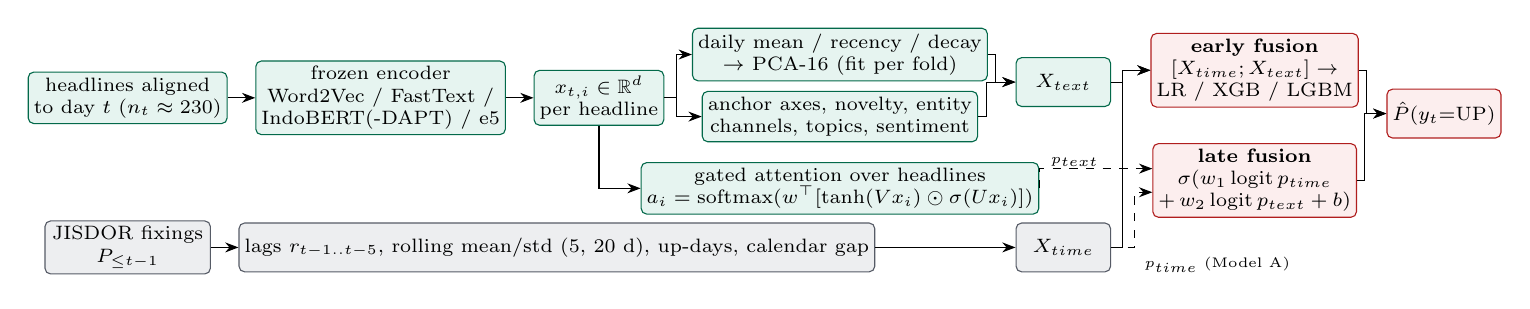
\begin{tikzpicture}[font=\scriptsize, >=Stealth,
  box/.style={draw, rounded corners=2pt, align=center, minimum height=0.62cm, inner sep=2pt},
  t/.style={box, fill=textc!10, draw=textc!70!black},
  m/.style={box, fill=timec!12, draw=timec!80!black},
  f/.style={box, fill=fusec!8, draw=fusec!80!black}]
% text branch
\node[t, minimum width=2.1cm] (h) at (0,1.9) {headlines aligned\\to day $t$ ($n_t\approx230$)};
\node[t, minimum width=2.3cm, right=0.35cm of h] (enc) {frozen encoder\\Word2Vec / FastText /\\IndoBERT(-DAPT) / e5};
\node[t, minimum width=1.6cm, right=0.35cm of enc] (vec) {$x_{t,i}\in\mathbb{R}^{d}$\\per headline};
\node[t, minimum width=3.0cm, right=0.35cm of vec, yshift=0.55cm] (agg) {daily mean / recency / decay\\$\to$ PCA-16 (fit per fold)};
\node[t, minimum width=3.0cm, below=0.12cm of agg] (named) {anchor axes, novelty, entity\\channels, topics, sentiment};
\node[t, minimum width=1.2cm, right=0.35cm of agg, yshift=-0.35cm] (xt) {$X_{text}$};
% time branch
\node[m, minimum width=2.1cm] (p) at (0,0) {JISDOR fixings\\$P_{\le t-1}$};
\node[m, minimum width=5.2cm, right=0.35cm of p] (tf) {lags $r_{t-1..t-5}$, rolling mean/std (5, 20 d), up-days, calendar gap};
\node[m, minimum width=1.2cm] (xm) at (xt |- tf) {$X_{time}$};
% fusion
\node[f, minimum width=2.4cm, right=0.5cm of xt, yshift=0.15cm] (early) {\textbf{early fusion}\\$[X_{time};X_{text}]\to$\\LR / XGB / LGBM};
\node[f, minimum width=2.4cm, below=0.45cm of early] (late) {\textbf{late fusion}\\$\sigma(w_1\,\mathrm{logit}\,p_{time}$\\$+\,w_2\,\mathrm{logit}\,p_{text}+b)$};
\node[f, minimum width=1.3cm, right=0.35cm of early, yshift=-0.55cm] (y) {$\hat P(y_t{=}\mathrm{UP})$};
% MIL
\node[t, minimum width=3.0cm, below=0.25cm of named] (mil) {gated attention over headlines\\$a_i=\mathrm{softmax}(w^\top[\tanh(Vx_i)\odot\sigma(Ux_i)])$};
\draw[->] (h) -- (enc); \draw[->] (enc) -- (vec);
\draw[->] (vec.east) -- ++(0.15,0) |- (agg.west); \draw[->] (vec.east) -- ++(0.15,0) |- (named.west);
\draw[->] (vec.south) |- (mil.west);
\draw[->] (agg.east) -- ++(0.1,0) |- (xt.west); \draw[->] (named.east) -- ++(0.1,0) |- (xt.west);
\draw[->] (p) -- (tf); \draw[->] (tf) -- (xm);
\draw[->] (xt.east) -- ++(0.15,0) |- (early.west); \draw[->] (xm.east) -- ++(0.15,0) |- (early.west);
\draw[->, dashed] (xm.east) -- ++(0.3,0) |- ([yshift=-0.15cm]late.west);
\node[font=\tiny, anchor=north west] at ([xshift=0.3cm]xm.east) {$p_{time}$ (Model A)};
\draw[->, dashed] (mil.east) -- ([yshift=0.15cm]late.west -| mil.east) -- ([yshift=0.15cm]late.west);
\node[font=\tiny, anchor=south] at ([xshift=0.45cm,yshift=0.15cm]mil.east) {$p_{text}$};
\draw[->] (early.east) -- ++(0.1,0) |- (y.west); \draw[->] (late.east) -- ++(0.1,0) |- (y.west);
\end{tikzpicture}}
\caption{Multimodal architecture. Text branch (green): every headline is encoded by a frozen encoder; vectors are aggregated per day (and compressed with PCA fitted on the fold's training days) or summarised by named features. Time branch (grey): 11 past-only rate features. \textbf{Early fusion} concatenates $X_{time}$ and $X_{text}$ into one classifier (all Model C rows). \textbf{Late fusion} trains unimodal models separately --- Model A for $X_{time}$, and a text-only LR or a gated-attention multiple-instance network over the day's headline stream for $X_{text}$ --- and stacks their logits; the stacker weights are fitted walk-forward on out-of-fold predictions only.}
\label{fig:arch}
\end{figure}
Figure~\ref{fig:arch} shows how text and numeric vectors are merged. In \emph{early fusion} (all Model~C rows) the day's text vector is concatenated with the 11 market features and passed to logistic regression, XGBoost or LightGBM; trees can model interactions such as ``negative geopolitical news matters only when recent volatility is high''. In \emph{late fusion} each modality has its own sub-model. The text sub-network is a gated-attention multiple-instance model (Ilse et al., 2018): the 128 headlines closest to the fixing are standardised, scored by an attention gate, and their attention-weighted projection (32 dims, $\approx$50k parameters, encoder frozen) gives $p_{text}$; the attention weights expose which headlines drove a prediction. A logistic stacker combines $\mathrm{logit}\,p_{time}$ and $\mathrm{logit}\,p_{text}$; for CV block $k$ its weights are fitted on the OOF predictions of blocks $<k$, so it never sees the days it scores. End-to-end fine-tuning of a 110--278M-parameter encoder on $\sim$800 labelled days was ruled out as it would memorise days: even our 50k-parameter attention model reached train AUC 0.94--0.99 with validation AUC $\approx$0.5 until heavily regularised.

\section{(c) Ablation matrix and discussion}
\begin{table}[t]
\centering\footnotesize
\setlength{\tabcolsep}{3pt}
\caption{Ablation matrix (Task~3 protocol). For each row, the model family with the best OOF AUC is shown (selection uses development data only). OOF: 600 out-of-fold days; test: 176 held-out days, evaluated once. Brackets: 95\% block-bootstrap CI; $\Delta$: paired bootstrap against Model~A of the same family. MCC at $P\ge0.5$.}
\label{tab:abl}
\resizebox{\textwidth}{!}{\begin{tabular}{@{}l l l c c c c c@{}}
\toprule
\textbf{Row} & \textbf{Features} & \textbf{Model} & \textbf{OOF AUC} & \textbf{OOF $\Delta$AUC vs A} & \textbf{Test AUC} & \textbf{Test MCC} & \textbf{Test $\Delta$AUC vs A} \\
\midrule
\textbf{A} & 11 market features & LR & 0.526 & -- & 0.564 {\scriptsize[0.484, 0.641]} & +0.086 & -- \\
\textbf{B} & + volume, GDELT tone, InSet, TF-IDF/SVD & LR & 0.515 & -0.011 {\scriptsize[-0.049, +0.027]} & 0.530 {\scriptsize[0.449, 0.605]} & -0.003 & -0.034 {\scriptsize[-0.111, +0.034]} \\
\midrule
C\_word2vec & + Word2Vec SIF, PCA-16 & LR & 0.501 & -0.025 {\scriptsize[-0.066, +0.015]} & 0.521 {\scriptsize[0.433, 0.606]} & -0.007 & -0.044 {\scriptsize[-0.111, +0.025]} \\
C\_fasttext & + FastText SIF, PCA-16 & LR & 0.494 & -0.032 {\scriptsize[-0.072, +0.006]} & 0.537 {\scriptsize[0.452, 0.623]} & +0.054 & -0.027 {\scriptsize[-0.079, +0.029]} \\
C\_indobert & + IndoBERT mean, PCA-16 & LGBM & 0.514 & -0.005 {\scriptsize[-0.048, +0.038]} & 0.515 {\scriptsize[0.430, 0.599]} & +0.074 & -0.005 {\scriptsize[-0.090, +0.077]} \\
C\_dapt & + IndoBERT-DAPT mean, PCA-16 & LR & 0.520 & -0.006 {\scriptsize[-0.045, +0.032]} & 0.536 {\scriptsize[0.455, 0.621]} & +0.027 & -0.028 {\scriptsize[-0.093, +0.039]} \\
C\_e5 & + e5 mean, PCA-16 & LR & 0.489 & -0.037 {\scriptsize[-0.074, +0.002]} & 0.603 {\scriptsize[0.518, 0.680]} & +0.154 & +0.039 {\scriptsize[-0.029, +0.107]} \\
C\_sentiment & + BERT sentiment (4) & LGBM & 0.549 & +0.030 {\scriptsize[-0.003, +0.064]} & 0.538 {\scriptsize[0.455, 0.625]} & +0.045 & +0.018 {\scriptsize[-0.040, +0.074]} \\
\midrule
C\_e5\_recency & + e5 recency-weighted, PCA-16 & LGBM & 0.530 & +0.011 {\scriptsize[-0.039, +0.061]} & 0.566 {\scriptsize[0.474, 0.655]} & +0.157 & +0.047 {\scriptsize[-0.065, +0.155]} \\
C\_e5\_decay & + e5 decay $h{=}3$d, PCA-16 & XGB & 0.512 & -0.008 {\scriptsize[-0.043, +0.028]} & 0.560 {\scriptsize[0.488, 0.631]} & +0.105 & +0.033 {\scriptsize[-0.052, +0.121]} \\
\midrule
C\_anchors & + 24 anchor axes, novelty & LR & 0.549 & +0.023 {\scriptsize[-0.020, +0.066]} & 0.482 {\scriptsize[0.391, 0.574]} & -0.003 & -0.082 {\scriptsize[-0.174, +0.014]} \\
C\_entities & + 5 entity channels (20) & LR & 0.531 & +0.005 {\scriptsize[-0.038, +0.047]} & 0.637 {\scriptsize[0.568, 0.711]} & +0.218 & +0.073 {\scriptsize[-0.005, +0.147]} \\
C\_topics & + 30 BERTopic shares & LR & 0.519 & -0.007 {\scriptsize[-0.050, +0.036]} & 0.473 {\scriptsize[0.377, 0.566]} & +0.008 & -0.091 {\scriptsize[-0.181, -0.007]} \\
C\_gdelt & + 30 GDELT theme shares & XGB & 0.523 & +0.004 {\scriptsize[-0.045, +0.051]} & 0.519 {\scriptsize[0.416, 0.624]} & +0.078 & -0.009 {\scriptsize[-0.116, +0.094]} \\
C\_combo & + anchors, entities, topics, sentiment & LR & 0.540 & +0.014 {\scriptsize[-0.036, +0.063]} & 0.510 {\scriptsize[0.417, 0.601]} & +0.126 & -0.054 {\scriptsize[-0.156, +0.052]} \\
\midrule
C\_tuned & Optuna-tuned C & LR & 0.557 & +0.031 {\scriptsize[-0.015, +0.076]} & 0.533 {\scriptsize[0.451, 0.614]} & +0.048 & -0.031 {\scriptsize[-0.121, +0.065]} \\
\midrule
T\_e5 & e5 PCA-16 only & LR & 0.472 & -0.053 {\scriptsize[-0.114, +0.004]} & 0.599 {\scriptsize[0.517, 0.672]} & +0.131 & +0.035 {\scriptsize[-0.070, +0.135]} \\
T\_anchors & anchor axes only & LR & 0.540 & +0.014 {\scriptsize[-0.049, +0.075]} & 0.441 {\scriptsize[0.353, 0.532]} & -0.114 & -0.123 {\scriptsize[-0.236, -0.007]} \\
MIL\_e5 & attention over headlines & MIL & 0.466 & -0.059 {\scriptsize[-0.122, +0.000]} & 0.559 {\scriptsize[0.469, 0.645]} & +0.076 & -0.005 {\scriptsize[-0.137, +0.119]} \\
\midrule
L\_e5 & A $\oplus$ T-e5 (logit stack) & stack & 0.502 & -0.024 {\scriptsize[-0.062, +0.013]} & 0.458 {\scriptsize[0.378, 0.539]} & -0.044 & -0.107 {\scriptsize[-0.190, -0.020]} \\
L\_mil & A $\oplus$ attention (logit stack) & stack & 0.521 & -0.004 {\scriptsize[-0.029, +0.019]} & 0.490 {\scriptsize[0.399, 0.586]} & -0.017 & -0.074 {\scriptsize[-0.144, +0.001]} \\
\bottomrule
\end{tabular}
}
\end{table}

\begin{table}[t]
\centering\footnotesize
\begin{minipage}{0.43\textwidth}
\centering
\caption{Task~2 vs Task~3 protocol, test set.}
\label{tab:t2}
\setlength{\tabcolsep}{3pt}
\begin{tabular}{@{}l l c c c c@{}}
\toprule
\textbf{Variant} & \textbf{Model} & \textbf{AUC} & \textbf{MCC} & \textbf{Acc} & \textbf{UP\%} \\
\midrule
Task 2 A & LR & 0.569 & +0.034 & 0.523 & 0.53 \\
Task 2 A & XGB & 0.533 & +0.177 & 0.625 & 0.90 \\
Task 2 B & LR & 0.504 & -0.006 & 0.489 & 0.45 \\
Task 2 B & XGB & 0.579 & +0.101 & 0.602 & 0.90 \\
Task 3 A & LR & 0.564 & +0.086 & 0.551 & 0.55 \\
Task 3 A & XGB & 0.527 & -0.027 & 0.489 & 0.51 \\
Task 3 B & LR & 0.530 & -0.003 & 0.483 & 0.41 \\
Task 3 B & XGB & 0.544 & +0.062 & 0.540 & 0.55 \\
\bottomrule
\end{tabular}

\end{minipage}\hfill
\begin{minipage}{0.55\textwidth}
\centering
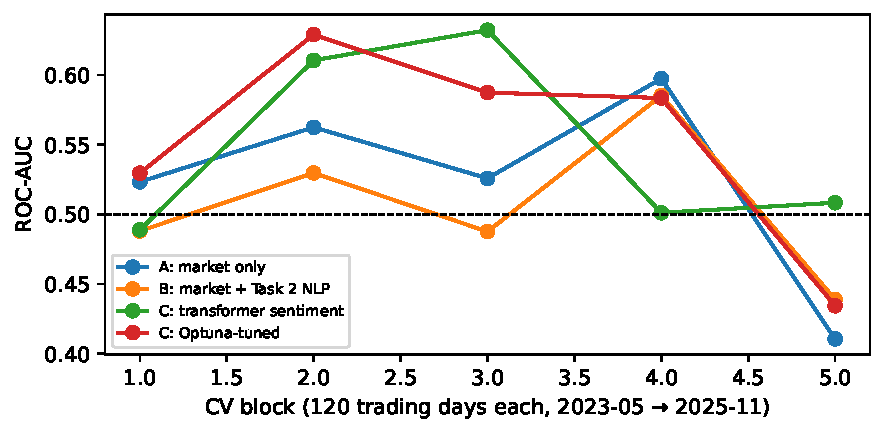
\includegraphics[width=\textwidth]{figures/fold_stability.pdf}
\captionof{figure}{OOF AUC per 120-day CV block (best model per row). Every row falls to $\approx$0.5 or below in some block, and the ranking changes from block to block.}
\label{fig:folds}
\end{minipage}
\end{table}

Table~\ref{tab:abl} is the full ablation; Table~\ref{tab:t2} contrasts the Task~2 numbers with the same models under the Task~3 protocol.
\begin{itemize}
\item \textbf{A vs B vs C.} The market-only Model~A reaches OOF AUC 0.526 and test AUC 0.564 (LR). Task~2's NLP features (B) do not help (test $\Delta$AUC $-0.034$). \textbf{No Model~C variant improves on A with a CI excluding zero}, on either evaluation (\NSigBetter{} of \NRows{} variants); \NSigWorse{} variants are significantly \emph{worse} on test. Task~2's best number (XGBoost A, MCC 0.177) was a validation artefact: under the new protocol the same model scores MCC $-0.027$.
\item \textbf{Representations.} Static embeddings (Word2Vec/FastText) and general IndoBERT are at chance OOF. e5 and its recency/decay variants obtain some of the best \emph{test} AUCs (0.56--0.60, $\Delta\approx+0.03$ to $+0.05$) but are \emph{below} A out-of-fold; the transformer sentiment head and the anchor axes are the best OOF rows (0.549) but do not transfer to test. Domain adaptation cuts held-out perplexity from \PplGeneral{} to \PplDapt{} and moves IndoBERT only marginally (OOF 0.514$\to$0.520, test 0.515$\to$0.536), within noise. The entity channels give the highest test AUC (0.637, MCC 0.218, $\Delta$ CI $[-0.005, 0.147]$) but only 0.531 OOF.
\item \textbf{Instability is the main result.} Across all variants, OOF and test AUC are uncorrelated (Spearman $\rho=\RhoOofTest$): whichever representation looks best on one period is not the best on the next (Fig.~\ref{fig:folds}). With $\pm0.08$ CI half-widths on 176 days, test differences of 0.03--0.07 between text representations are indistinguishable from noise.
\item \textbf{Fusion.} Late fusion did not help: because the text-only models were \emph{anti}-predictive out-of-fold (attention model OOF AUC 0.466, e5 LR 0.472), the stacker learned negative text weights ($w_{text}=\WtextMil$ for attention, $\WtextE$ for e5), which then hurt on test, where the same text models were mildly positive --- a regime flip, not a modelling bug.
\item \textbf{Tuning.} Optuna (\TunedTrials{} TPE trials) searched PCA size, extra feature groups, model family and hyper-parameters around the two best OOF rows (\TunedStart). The best trial reached OOF AUC \TunedOof{} (optimistic: selected on those days) but test AUC \TunedTest{} ($\Delta$ vs A $\TunedTestD$), confirming that more search fits OOF noise.
\end{itemize}

\section{(d) Exploratory analysis}
\begin{figure}[t]
\centering
\begin{subfigure}[b]{0.36\textwidth}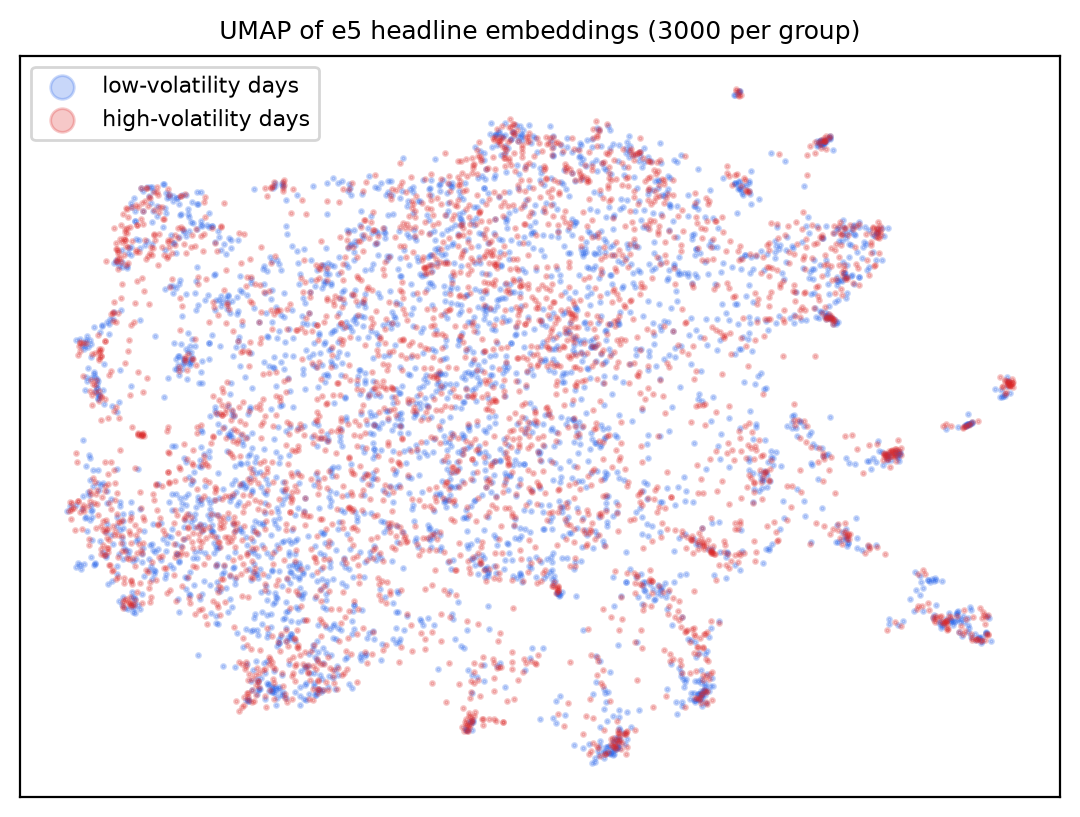
\includegraphics[width=\textwidth]{figures/umap_volatility.png}\caption{UMAP of e5 headline vectors.}\end{subfigure}\hfill
\begin{subfigure}[b]{0.62\textwidth}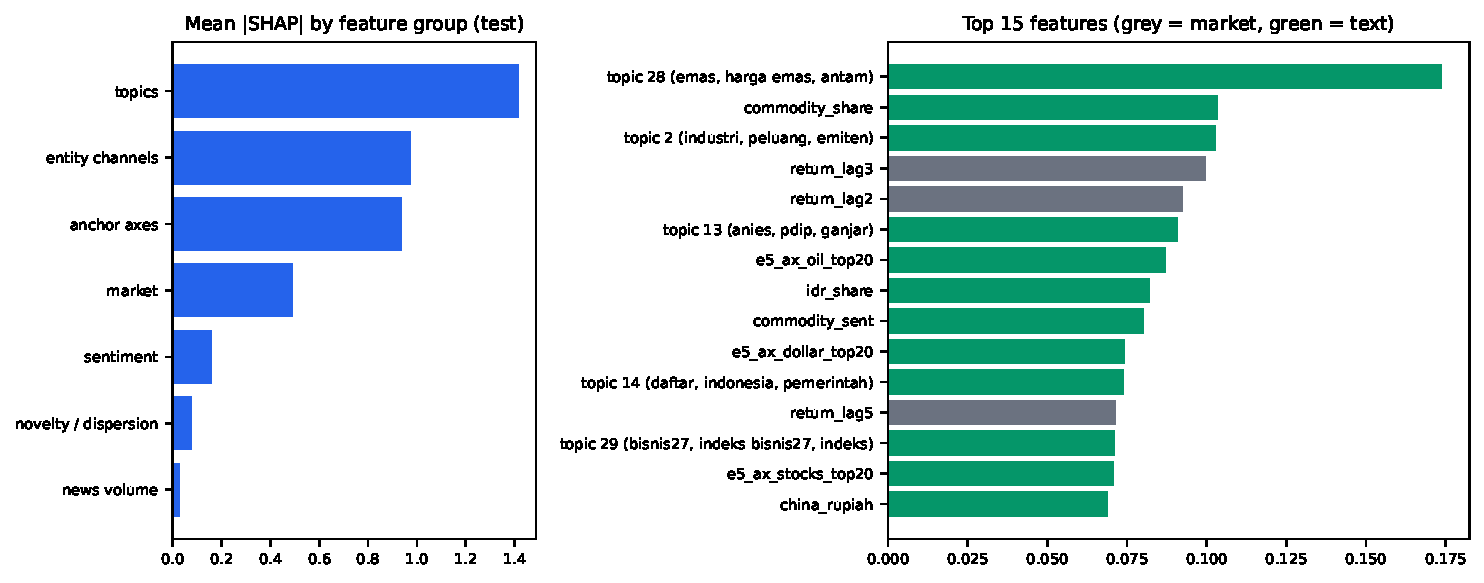
\includegraphics[width=\textwidth]{figures/shap_groups.pdf}\caption{TreeSHAP of the named-feature Model C (test days).}\end{subfigure}\\[2pt]
\begin{subfigure}[b]{0.49\textwidth}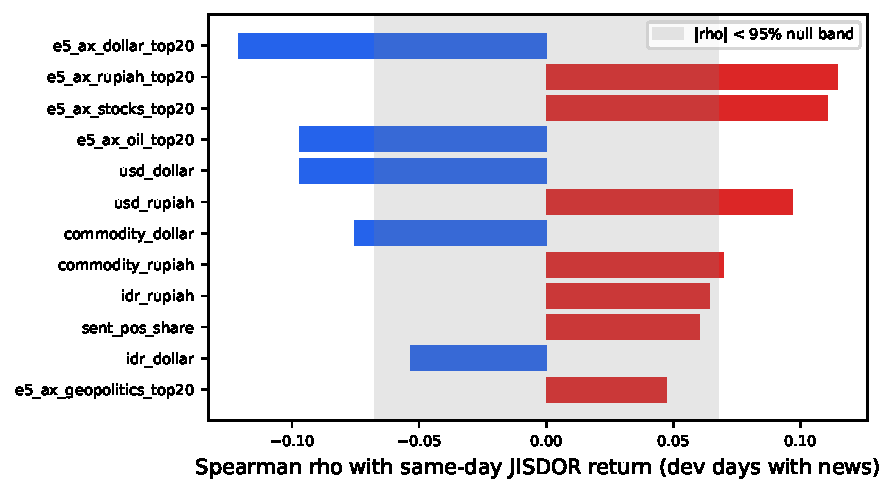
\includegraphics[width=\textwidth]{figures/feature_correlations.pdf}\caption{Spearman $\rho$ of text features with the same-day return.}\end{subfigure}\hfill
\begin{subfigure}[b]{0.49\textwidth}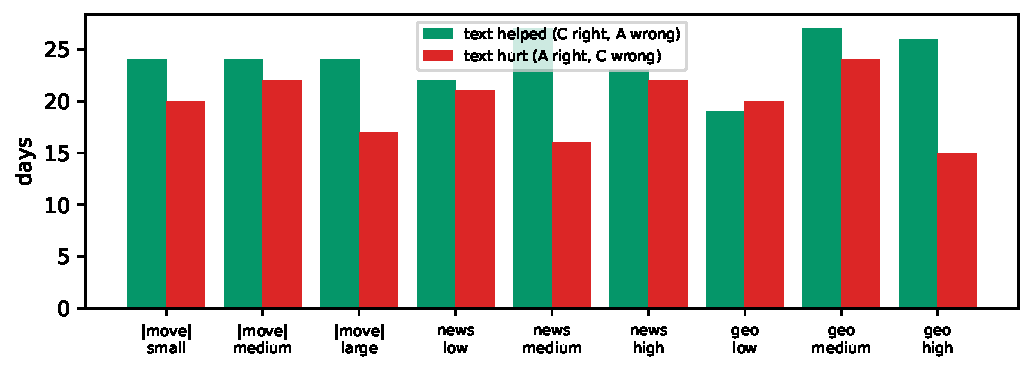
\includegraphics[width=\textwidth]{figures/error_breakdown.pdf}\caption{Days where text helped vs hurt (OOF), by tercile.}\end{subfigure}
\caption{Exploratory analysis of the text features (notebooks 04--06).}
\label{fig:explore}
\end{figure}
\textbf{Embedding space (high vs low volatility).} Headlines on the top-quintile $|r_t|$ days are not a separate cluster in UMAP space (Fig.~\ref{fig:explore}a); a classifier on daily mean embeddings separates high- from low-volatility days with AUC 0.60--0.63 (e5 0.631, IndoBERT-DAPT 0.619 $>$ general IndoBERT 0.596), but these days cluster in time, so part of this is era rather than content: Covid-19 and Russia--Ukraine topics are over-represented on \emph{low}-volatility days, election, banking and infrastructure topics --- and, more mildly, the Fed and Israel--Gaza topics --- on high-volatility days (notebook 04).

\textbf{What drives the predictions.} TreeSHAP on the named-feature Model C (Fig.~\ref{fig:explore}b) attributes the largest single contributions to the gold-price topic (T28), commodity and IDR-side channel shares, lagged returns, and the oil and dollar anchor axes. The largest test-day shifts away from Model~A are traceable to specific news: e.g.\ on 2026-08-03 Model~A said UP (0.65) while Model~C said DOWN (0.25), driven by the USD channel with headlines ``\emph{Rupiah Dibuka Menguat \dots Terangkat Data Ekonomi AS}'' --- the rupiah did strengthen; on 2026-01-22 a record gold price (commodity channel) pushed C towards UP on a DOWN day.

\textbf{Correlation and error analysis.} Text features \emph{are} related to the move being forecast: the top-20 ``rupiah weakens'' axis correlates positively with the same-day JISDOR return ($\rho=+0.115$, $p<0.001$, $n=848$), as do the USD-channel rupiah axis and the stock-market axis (Fig.~\ref{fig:explore}c). The pre-fixing morning headlines partly report the spot market's opening (``\emph{Rupiah dibuka melemah}''), which is genuine information before 10:00. Counter-intuitively the dollar axis has the opposite sign, which suggests that e5's cosine geometry does not cleanly separate the two currencies' directions. The effects are $|\rho|\le0.12$, i.e.\ at most $\sim$1.5\% of variance. Comparing the best OOF Model~C (sentiment, LightGBM) with Model~A of the same family, the two disagree on 131 of 600 OOF days: text turned a wrong market call into a right one on 72 days and the reverse on 59 (test: 26 vs 20). The net benefit is concentrated on days with a high share of geopolitical news ($+11$ days in the top tercile vs $-1$ in the bottom) and on large-move days (Fig.~\ref{fig:explore}d). Typical ``helped'' days carry pre-fixing spot-market headlines --- 2024-10-07: ``\emph{Rupiah Dibuka Melemah ke Level Rp15.52, Mayoritas Mata Uang Asia Memerah}'' (USD/IDR $+1.19\%$); typical ``hurt'' days mix contradictory Fed and rupiah news (2024-08-26, Jackson Hole).

\section{Conclusion and limitations}
Transformer and embedding features did \emph{not} measurably improve daily JISDOR direction forecasting over exchange-rate history in this dataset: all differences to Model~A lie within bootstrap uncertainty, and the ranking of representations is not stable between periods. The rigorous protocol is what makes this visible --- a single test split would have crowned e5 (AUC 0.603) or entity channels (0.637). The text is informative about the \emph{same-day} move but the signal is small, partly already priced by the previous fixing, and non-stationary. Limitations: Indonesian outlets only (the GDELT quota prevented global English news), a 2022--23 coverage gap, bodies only for 2024 (title vs body could not be compared over the full period), and frozen encoders. Task~4 will test the hypothesis formally (e.g.\ Diebold--Mariano and permutation tests on the OOF predictions) and examine intraday-aligned text.

\vspace{-0.3em}
{\footnotesize \textbf{References.} Gururangan et al.\ (2020) Don't Stop Pretraining, ACL. Arora et al.\ (2017) A Simple but Tough-to-Beat Baseline for Sentence Embeddings, ICLR. Ilse et al.\ (2018) Attention-based Deep Multiple Instance Learning, ICML. Wang et al.\ (2022) Text Embeddings by Weakly-Supervised Contrastive Pre-training (E5). Wilie et al.\ (2020) IndoNLU, AACL. Grootendorst (2022) BERTopic. Lundberg \& Lee (2017) SHAP, NeurIPS.}

\end{document}
